\begin{figure}
	\centering
	\begin{tikzpicture}[
		scale=0.6
	]
		
		\node[align=center] at (-10,0) {$\mathcal{X}$ \\ \tiny Input space};
		\node (X) at (-5,0) {
			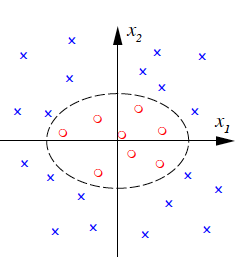
\includegraphics[scale=0.5]{11_svm/02_img/input_space}
		};

		\node[align=center] at (10,0) {$\mathcal{F}$ \\ \tiny Feature space};
		\node (F) at (5,0) {
			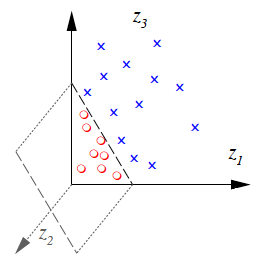
\includegraphics[scale=0.5]{11_svm/02_img/feature_space}
		};

		\draw[->,ultra thick] (X) -- node[above] {$\varphi : \mathcal{X} \mapsto \mathcal{F}$} (F);
		
	\end{tikzpicture}
\end{figure}